\documentclass[11pt]{article}
\author{Tarang Srivastava}
\usepackage{amsmath,amsthm}
\usepackage{chngcntr}                                   
\theoremstyle{definition}
\newtheorem{example}{Example}
\counterwithin*{example}{subsection} 
\usepackage{graphicx}
\usepackage{multicol}
\usepackage{esdiff}
\usepackage[margin=1in]{geometry}

\begin{document}
	\begin{titlepage}
		\begin{center}
			\vspace*{1cm}
			\Huge
			\textbf{Differential Equations}\\
			\vspace{0.5cm}
			\LARGE
			A Concise Review of Elementary Differential Equations\\
			\vspace{1.5cm}
			\textbf{Tarang Srivastava}\\
			\vfill
			\vspace{0.8cm}
			\Large
			Dr. Mesut Cakir\\
			Differential Equations and Complex Analysis\\
			South Brunswick High School\\
			14 February 2018
			
		\end{center}
	\end{titlepage}
	\tableofcontents	
	\pagebreak
	\section{Introduction}
	\subsection{Basic Mathematical Models}
	In this concise review we will provide brief explanations to the core concepts of differential equations, and include some examples to show the many techniques used in differential equations. Refer to the scratch paper if further examples and procedures are needed. For future reference the textbook used is "Elementary Differential Equations and Boundary Value Problems" by William E. Boyce and Richard C. DiPrima. All the graphics used in this document were created by Tarang Srivastava in Wolfram Mathematica \\
	
	Equations considering derivatives are \textbf{differential equations}. A differential equation that describes a physical process is a \textbf{mathematical model}. \\
	A model for an object falling in earth's atmosphere may be given by the differential equation $m \frac{dv}{dt} = mg - \gamma v$. Moving things around we get $\frac{dv}{dt} = 9.8 - \frac{v}{5}$ There are several solutions for this equation and can be represented by the slope field. \\
	\begin{center}
		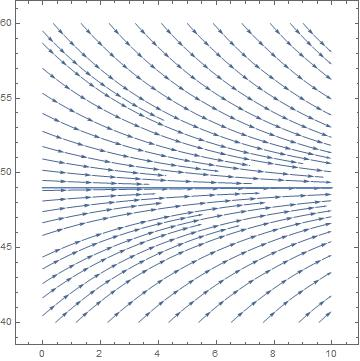
\includegraphics[width=10cm]{f1}
		$$\frac{dv}{dt} = 9.8 - \frac{v}{5}$$
	\end{center}
	The line $y=49$ shows the equilibrium solution for this case\\
	\subsection{Solutions of Differential Equations}
	When a problem is given where there are infinite solutions, usually when there is a constant in the solution as a result of integration, an \textbf{initial condition} can be set to find a particular answer, this is called an \textbf{initial value probelm}. A general example of this is
	\begin{align*}
	\dfrac{dy}{dt} = ay - b \\
	y(0) = y_0 \\
	\frac{dy/dt}{y-(b/a)} = a\\
	\ln{ \vline y-(b/a) \vline} = at + C && \text{Where C is an arbitrary constant}\\ 
	y = b/a + ce^{at} && \text{solve for C using the initial condition}\\
	y = b/a + (y_0 - b/a)e^{at}
	\end{align*}
	The \textbf{general solution} with the constant gives all possible solutions, and graphs the \textbf{integral curves} 
	\begin{center}
		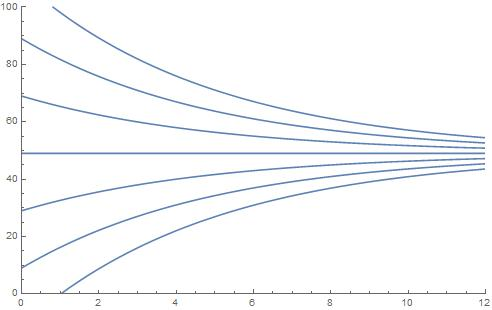
\includegraphics[width=12cm]{f2}
	\end{center}
	$$v = 49 + ce^{-t/5}$$
	\subsection{Classification of Differential Equations}
	Differential equations are classified into \textbf{ordinary differential equations} and \textbf{partial differential equations}. ODE have ordinary derivatives whereas PDE have partial derivatives. The \textbf{order} is the highest derivative. There are linear and nonlinear functions, we will mostly deal with linear for now. 
	\pagebreak
	\section{First Order Differential Equations}
	We will focus on differential equations of first order 
	$$\diff{y}{t} = f(t,y)$$
	One of the notations used is that for any differentiable function $y=\phi(t)$ that satisfies the differential equation. 
	\subsection{First Order Linear Equation}
	$$P(t) \diff{y}{t} + Q(t)y = G(t)$$
	This gives a standard form for solving linear equations. To solve such linear equations, we use a \textbf{integrating factor} $\mu(t)$. \\
	\begin{example}
		Find the general solution of the differential equation
		\begin{align}
		\diff{y}{t} + \frac{1}{2} y = \frac{1}{2}e^{t/3} \\
		\mu(t)\diff{y}{t} + \mu(t)\frac{1}{2} y = \mu(t)\frac{1}{2}e^{t/3} && \text{we multiply by the integrating factor} \\
		\diff{}{t}[\mu(t)y] = \mu(t)\diff{y}{t} + \diff{\mu(t)}{t} y && \intertext{We notice that the first part on the right side of (3) exists as the first part in (2)}\\
		\diff{\mu(t)}{t} = \frac{1}{2} \mu(t)\\
		\frac{d\mu(t)/dt}{\mu(t)} = \frac{1}{2}\\
		\diff{}{dt} \ln \vline \mu(t) \vline = \frac{1}{2}\\
		\ln \vline \mu(t) \vline = \frac{1}{2}t + C && Integrating follows\\
		\mu(t) = c e^{t/2} && \intertext{Any value for c (obviously not 0) can be used to find the integrating factor. Since there are multiply integrating factors that would suffice, so we use $c = 1$} \\
		e^{t/2}\diff{y}{t} + \frac{1}{2}e^{t/2}y = \frac{1}{2}e^{5t/6} \\ 
		\diff{}{t} \left( e^{t/2} y\right) = \frac{1}{2}e^{5t/6} && \text{This was the whole point of using $\mu(t)$}\\
		\left( e^{t/2} y\right) = \frac{3}{5}e^{5t/6} + c && \text{from integrating both sides}\\
		y = \frac{3}{5}e^{t/3} + ce^{-t/2} && \text{Solving for y}\\
		\intertext{This is the general solution. Huzzah! Lets say we have to find a solution that goes through point (0,1) then we solve for c by setting $y=1$ and $t=0$}
		y = \frac{3}{5}e^{t/3} + \frac{2}{5}e^{-t/2} && \text{This is also the initial value solution}
		\end{align}
	\end{example}
	
	
	\begin{center}
		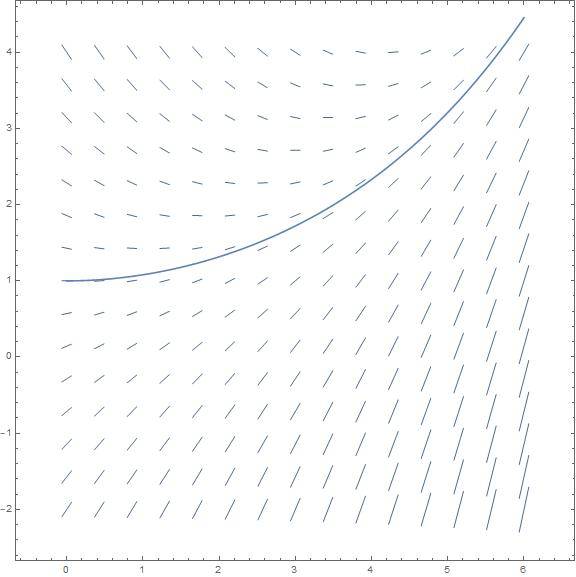
\includegraphics[width=10cm]{f3}\\
		Here is a graph of the slope field(1) and the initial value solution(15). 
	\end{center}
	\subsection{Separable Equations}
	These are generally the easiest differential equations to solve, as they require a simple rearrangement and then integration. Though you should consider possibly the intervals in which a solution exists, especially when you are given an initial value condition, since you may obtain two (or more) general solution and you have to find the one that contains the initial value. \\
	Separable equations are equations of the form $$M(x) dx + N(y)dy = 0$$ 
	\begin{example} Solve the initial value problem, and determine the interval in which the solution exists. 
		\begin{align*}
		\diff{y}{x} = \frac{3x^2+4x+2}{2(y-1)}, && y(0) = -1 
		\intertext{The equation can be rewritten as}
		2(y-1)dy = (3x^2+4x+2)dx 
		\intertext{Integrating the left side with respect to y, and the right side with respect to x}
		y^2-2y = x^3 + 2x^2 +2x+c 
		\intertext{solving for c using the initial coniditon $x=0$ and $y=-1$ and get $c = 3$. The solving for y in terms of x, we complete the square and find}
		y = 1 \pm \sqrt{x^3 + 2x^2 + 2x+4} 
		\intertext{considering the initial value condition only the $	y = 1 - \sqrt{x^3 + 2x^2 + 2x+4}$ satisfies the conidition }
		\end{align*}
	\end{example}
	
	
%	\subsection{Modeling with First Order Equations}
	This should be an important focus on anyone trying to learn Differential Equations, and effectively use it. Personally, I believe this is the hardest part and the most useful part of this subject. We will study several examples that deal with modeling, and there are a couple of basic tricks we will understand when learning to model differential equations. 
	\begin{example}
%		 
		At time $t = 0$ a tank contains $Q_0$ lb of salt dissolved in 100 gal of water; Assume that water containing $\dfrac{1}{2}$ lb of slat/gal is entering the tank at a rate of $r$ gal/min, and that well-stirred mixture is draining from teh tank at the same rate. Set up the initial value problem that describes this flow process. Find the amount of salt $Q(t)$ in the tank at any time, and also find the limiting amount $Q_L$ that is present after a very long time. If $r=3$ and $Q_0=2Q_L$, find the time $T$ after which the salt level is within $2\%$ of $Q_L$. Also find the flow rate required if the value of $T$ is not to exceed 45 min.\\ \begin{center}
			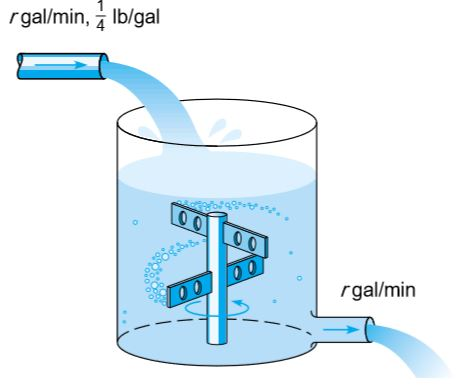
\includegraphics[width=10cm]{figure231} 
		\end{center} 
		\begin{multicols}{2}
			\begin{align}
			\diff{Q}{t} = \text{rate in} - \text{rate out} 
			\intertext{salt enters at  $\dfrac{1}{4}$ lb/gal times the flow rate $r$ gal/min. Also volume is constant, and concentration is uniform}
			\diff{Q}{t} = \dfrac{r}{4} - \dfrac{rQ}{100}
			\intertext{The initial condition is}
			Q(0) = Q_0
			\intertext{rearragning to}
			\diff{Q}{t} = \dfrac{rQ}{100} = \dfrac{r}{4}
			\intertext{solving for the genral solution with the integrating factor $e^{rt/100}$ we find}
			Q(t) = 25 + ce^{-rt/100}
			\intertext{Using the initial condition we find the initial solution to be}
			Q(t) = 25 + (Q_0-25)e^{-rt/100}
			\intertext{$Q(t) \rightarrow 25 $ as $t \rightarrow \inf$ so the limiting value} 
			Q_L = 25
			\end{align}
		\end{multicols}
		\begin{figure}[h]
			\centering
			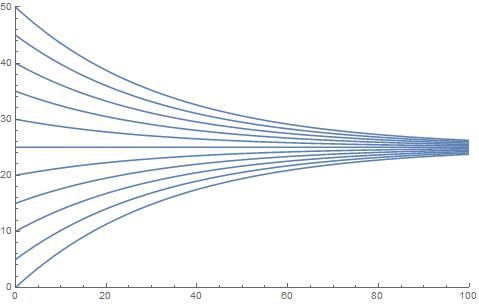
\includegraphics[width=10cm]{Model1}
			\caption{Several plots for the general solution (20) for Example 3}
			Considering Figure 1 we see that the values converge to 25, which supports that $Q_L = 25$
		\end{figure}
		
	\end{example}
	In the previous example te rate in and out did not vary, we will consider a similar example in which it does vary. This does not make the problem more difficult, but we will study this behavior in the graph of the initial solution. 
	\begin{example}
		
		Consider a pond that initially contains 10 million gal of fresh water. Water containing an undesirable chemical flows into the pond at the rate of 5 million gal/year and the mixture in the pond flows out into the pond at the rate of 5 million gal/year and the mixture in the pond flows out at the same rate. The concentration $\gamma (t)$ of chemical in the incoming water varies periodically with time according to the expression $\gamma(t) = 2 + \sin 2t g/gal$. Construct a mathematical model of this flow process and determine the amount of chemical in the pond at any time. Plot the solution and describe in words the effect of the variation in the incoming concentration. Since the incoming and outgoing flows of water are the same, the amount of water int eh pond remains constant at $10^7$ gal. Let us denote time by $t$, measured in years, and the chemical by $Q(t)$, measured in grams. This example is similar to Example 1 and the same inflow/outflow principle applies. 
		\begin{align*}
		\diff{Q}{t} = \text{rate in} - \text{rate out}, \\
		\text{rate in} = (5 \times 10^6)(2+\sin 2t) 
		\intertext{The concentration of chemical in the pond is $Q(t)/10^7$, so the rate of flow out is}
		\text{rate out} = (5 \times 10^6)(Q(t)/10^7) = Q(t)/2 \\
		\diff{Q}{t} = (5 \times 10^6)(2 + 2\sin 2t )- \dfrac{Q(t)}{2} 
		\intertext{to make the work more easy lets introuduce $q(t) = Q(t)/10^6$}
		\diff{q}{t} + \dfrac{1}{2}q = 10 + 5 \sin 2t
		\intertext{the initial condition is}
		q(0) = 0 
		\intertext{the integrating factor is $e^{t/2}$}
		q(t) = 20-\dfrac{40}{17}\cos 2t + \dfrac{10}{17} \sin 2t + ce^{-t/2}
		\intertext{solving for the initial condition}
		q(t) = 20-\dfrac{40}{17}\cos 2t + \dfrac{10}{17} \sin 2t - \dfrac{300}{17}e^{-t/2}
		\end{align*}
		\begin{figure}[h]
			\centering
			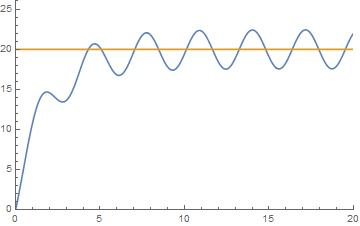
\includegraphics[width=10cm]{Model2}
			
		\end{figure}
		
	\end{example}
	\pagebreak
	\subsection{Differences Between Linear and Nonlinear Equation}
	Let the functions of $f$ and $\partial f / \partial y$ be continuous in some rectangle $\alpha < t < \beta$, $\gamma < y < \delta$ containing the point $(t_0,y_0)$. Then in some interval $t_0-h<t<t_0+h$ contained in $\alpha < t < \beta $, there is a unique solution $y=\phi (t)$ of an initial value problem
	\begin{example}
		Find the interval of the initial value problem 
		\begin{align*}
		ty' + 2y = 4t^2 \\
		y(1) = 2 \\
		y' = (2/t)y = 4t 
		\intertext{Referring to the form $y' + p(t)y = g(t)$ we find that $p(t) = 2/t$ and $g(t) = 4t$. $g(t)$ is continuous everywhere but $p(t)$ is only continuous in $(-\infty, 0)\cup (0,\infty)$ Since the ininitial value gives that $y(1) = 2$, we know that the equation exists in the interval, and has a unique solution}
		y = t^2 + \dfrac{1}{t^2}, && t>0
		\end{align*}
	\end{example}
%	\subsection{Autonomous Equations and Population Dynamics}
	We will consider a specific example on how to derive the equation for carrying capacity, and population dynamics of a species
	\begin{align*}
	dy/dt = f(y) && \text{This is the form we will consider} \\
	dy/dt = ry 
	\intertext{if we subject it to an initial condition}
	y(0) = y_0 \\
	y = y_0 e^{rt}
	\intertext{Now to actually show that growth rate depends on population, we get}
	dy/dt = h(y)y && \text{Replacing $r$ with $h(y)$} \\
	dy/dt = (r-ay)y 
	\intertext{This represents the population growth. We rewrite it as}
	\diff{y}{t} = r\left( 1 - \dfrac{y}{K}\right)y && \text{Where $K = r/a$}
	\intertext{The simplest form is where growth is constant so $dy/dt = 0$. This gives}
	r(1-y/K)y = 0
	\intertext{This gives the two equilibrium solutions}
	y = \phi _1 (t) = 0 \\
	y = \phi _2 (t) = K 
	\intertext{Using techniques in the earlier sections we can find the solution to when the growth rate is not constant. We separate the earlier equation and get}
	\dfrac{dy}{(1-y/K)y} = r dt
	\intertext{Use partial fraction seperation}
	\left( \dfrac{1}{y} + \dfrac{1/K}{1-y/K}\right)dy = rdt
	\intertext{Integrate both sides}
	\ln |y| - \ln |1-\dfrac{y}{K}| = rt + c
	\intertext{Solving for y, and the constant we get}
	y = \dfrac{y_0K}{y_0 + (K-y_0)e^{-rt}} && \text{This is the solution for such a differential equation}
	\end{align*}
	\subsection{Exact Equations and Integrating Factors}
	This is fun. We will discuss another method for solving first order differential equations in very special cases 
		\begin{example}
		Solve the differential equation
			\begin{align*}
				2x + y^2 +2xyy' = 0
				\intertext{We seperate the equation into two parts such}
				M(x,y) = 2x + y^2 \\
				N(x,y) = 2xy\\
				M + Ny' = 0
				\intertext{Now we show that}
			\end{align*}
		\end{example}
	\end{document}

